\documentclass[11pt,letterpaper]{article}

\usepackage[utf8]{inputenc}
\usepackage[spanish,es-nodecimaldot]{babel}
\usepackage[margin=2cm]{geometry}
\usepackage{amsmath,amssymb}
\usepackage{graphicx}
\usepackage{booktabs}
\usepackage{tabularx}
\usepackage{xcolor}
\usepackage{titlesec}
\usepackage{fancyhdr}
\usepackage{hyperref}
\usepackage{float}
\usepackage{microtype}

\definecolor{umesblue}{RGB}{20, 50, 100}
\definecolor{umesred}{RGB}{180, 40, 40}
\definecolor{darkgray}{RGB}{60, 60, 60}

\hypersetup{
    colorlinks=true,
    linkcolor=umesblue,
    urlcolor=umesblue,
    citecolor=umesblue
}

\pagestyle{fancy}
\fancyhf{}
\fancyhead[L]{\small \textbf{UMES} -- Proyecto Final de Estadística}
\fancyhead[R]{\small Análisis Acústico en Laboratorio de Prototipos}
\fancyfoot[C]{\thepage}
\renewcommand{\headrulewidth}{0.8pt}

\titleformat{\section}{\Large\bfseries\color{umesblue}}{\thesection.}{0.5em}{}[\titlerule]
\titleformat{\subsection}{\large\bfseries\color{darkgray}}{\thesubsection.}{0.5em}{}

\begin{document}

% ==============================================================================
% PORTADA / ENCABEZADO
% ==============================================================================
\begin{center}
    {\large \textbf{UNIVERSIDAD MESOAMERICANA SEDE QUETZALTENANGO}}\\[0.2cm]
    {\normalsize \textbf{FACULTAD DE INGENIERÍA -- INGENIERÍA EN SISTEMAS}}\\[0.4cm]
    {\small \textbf{Catedrático:} Ing. Josué Cifuentes \quad | \quad \textbf{Cátedra:} Estadística}\\[0.6cm]
    {\LARGE \textbf{\color{umesblue} Informe Técnico de Resultados y Memoria Estadística}}\\[0.3cm]
    {\large \textbf{Análisis de Ruido y Tendencias en el Laboratorio de Prototipos}}\\[0.5cm]
    \rule{\linewidth}{1.2pt}\\[0.3cm]
\end{center}

\vspace{-0.3cm}
\noindent\textbf{Nombre del Estudiante:} Arturo \hfill \textbf{Fecha de Análisis:} Noviembre 2026\\
\textbf{Sistema de Captura:} Microcontrolador ESP32 + Micrófono I2S INMP441\\
\textbf{Base de Datos:} Supabase PostgreSQL \hfill \textbf{Herramienta Estadística:} RStudio / R 4.4+
\vspace{0.2cm}
\rule{\linewidth}{0.6pt}

% ==============================================================================
% 1. INTRODUCCIÓN Y ARQUITECTURA DEL SISTEMA
% ==============================================================================
\section{Introducción y Contexto del Monitoreo}
El presente proyecto evalúa el comportamiento acústico y los patrones de ruido en el \textbf{Laboratorio de Prototipos de la Universidad Mesoamericana (UMES)}, contrastando las mediciones contra umbrales normativos de exposición y desarrollando modelos de regresión temporal y probabilidad binomial.

\subsection{Descripción del Entorno Físico}
El Laboratorio de Prototipos presenta la siguiente distribución operativa:
\begin{itemize}
    \item \textbf{3 Cubículos de Prototipado Especializado:} Estaciones de trabajo individuales o en parejas donde se instaló el nodo sensor ESP32 con micrófono digital INMP441. En ellos se realizan actividades de medición, programación y soldadura.
    \item \textbf{1 Salón Principal con 4 Mesas de Trabajo Colaborativo:} Espacio amplio destinado a proyectos grupales y ensamble mecánico con capacidad simultánea para aproximadamente \textbf{40 estudiantes}.
    \item \textbf{Dinámica de Ocupación:} El laboratorio presenta una concurrencia variable. El ruido ambiental combina la discusión técnica con maquinaria de prototipado rápido (impresoras 3D, fresadoras y fuentes de poder).
\end{itemize}

\subsection{Pipeline de Adquisición y Procesamiento de Datos}
El sistema de monitoreo opera mediante un pipeline continuo:
\begin{enumerate}
    \item \textbf{Adquisición Local:} El ESP32 captura audio PCM de 16 bits a 16 kHz mediante el micrófono I2S INMP441, calculando el valor eficaz (RMS) y la potencia relativa en decibeles escala digital ($\text{dBFS}$).
    \item \textbf{Servidor y Persistencia:} Los datos se transmiten vía WebSockets a un backend en Python (FastAPI/Uvicorn), el cual acumula las lecturas y registra cada 15 minutos en Supabase PostgreSQL el promedio de decibeles, el pico y el estado del umbral.
    \item \textbf{Estandarización Temporal (UTC a UTC-6):} El servidor almacena los registros con marca de tiempo UTC-0. El script de procesamiento en Python aplica la transformación a la hora oficial de Guatemala ($\text{UTC}-6$):
    \begin{equation}
        \text{Hora}_{\text{Guatemala}} = \text{Hora}_{\text{UTC}} - 6\text{ horas}
    \end{equation}
    \item \textbf{Calibración Acústica ($\text{dBFS} \rightarrow \text{dBA}$):} Dado que el INMP441 mide en decibeles fondo de escala digital ($\text{dBFS}$ negativos), se aplica la función de sonometría acústica equivalente:
    \begin{equation}
        \text{dBA} = \text{dBFS} + 105.0
    \end{equation}
    Bajo esta equivalencia, el umbral de $-40.0\text{ dBFS}$ corresponde con exactitud a $65.0\text{ dBA}$.
\end{enumerate}

% ==============================================================================
% 2. FASE 1: NORMATIVA Y AUDITORÍA
% ==============================================================================
\section{Fase 1: Recolección y Marco Normativo de Ruido}

\subsection{Definición del Umbral de Riesgo Aceptado}
Para determinar el criterio de exceso sonoro, se adoptaron los estándares de la \textbf{Organización Mundial de la Salud (OMS)}, la norma \textbf{ISO 1996} y la legislación laboral guatemalteca (\textbf{Acuerdo Gubernativo 229-2014}):
\begin{itemize}
    \item \textbf{Áreas de Estudio y Diseño Intelectual:} El límite óptimo se ubica en $55\text{ dBA}$.
    \item \textbf{Talleres Universitarios y Laboratorios Técnicos:} El umbral crítico de tolerancia se establece en \textbf{65.0 dBA} (equivalente a $-40.0\text{ dBFS}$). Superar este límite incrementa el estrés cognitivo, dificulta la inteligibilidad del habla y eleva la tasa de error.
\end{itemize}

\subsection{Auditoría de los Datos Extraídos de Supabase}
Se extrajeron un total de \textbf{236 registros reales} correspondientes a los 4 días de medición (del 3 al 6 de noviembre de 2026), capturados a intervalos de 15 minutos. El cuadro \ref{tab:resumen_dias} resume el comportamiento por día.

\begin{table}[H]
\centering
\caption{Resumen diario de mediciones acústicas en el Laboratorio de Prototipos (Hora local UTC-6).}
\label{tab:resumen_dias}
\vspace{0.2cm}
\begin{tabular}{l c c c c c}
\toprule
\textbf{Día de Monitoreo} & \textbf{Muestras} & \textbf{Media ($\text{dBA}$)} & \textbf{Pico Máx ($\text{dBA}$)} & \textbf{Excesos ($\ge 65\text{ dBA}$)} & \textbf{\% Exceso} \\
\midrule
Día 1 (2026-11-03, Jueves) & 36 & 63.88 & 104.85 & 22 & 61.11\% \\
Día 2 (2026-11-04, Viernes) & 62 & 58.79 & 105.00 & 5 & 8.06\% \\
Día 3 (2026-11-05, Sábado) & 96 & 54.46 & 95.59 & 4 & 4.17\% \\
Día 4 (2026-11-06, Domingo) & 42 & 48.82 & 93.13 & 0 & 0.00\% \\
\midrule
\textbf{Total / Promedio Global} & \textbf{236} & \textbf{56.03} & \textbf{105.00} & \textbf{31} & \textbf{13.14\%} \\
\bottomrule
\end{tabular}
\end{table}

\noindent\textbf{Interpretación Técnica del Comportamiento Diario:}
El Día 1 registró el mayor porcentaje de exceso ($61.11\%$) debido a que el monitoreo inició en horario de máxima actividad lectiva diurna (09:33 a 19:51 hrs) con pruebas de laboratorio. Por el contrario, los Días 3 y 4 incluyen extensos periodos nocturnos y de fin de semana (00:00 a 06:00 hrs) donde el laboratorio se mantuvo cerrado, registrando el piso acústico del edificio ($\approx 46\text{--}49\text{ dBA}$).

% ==============================================================================
% 3. FASE 2: ESTADÍSTICA DESCRIPTIVA Y PROYECCIÓN DÍA 6
% ==============================================================================
\section{Fase 2: Estadística Descriptiva y Proyección de Tendencia (Día 6)}

\subsection{Medidas de Tendencia Central y Dispersión Global}
A partir del total de $N = 236$ observaciones procesadas en RStudio, se obtuvieron los parámetros estadísticos muestrales descritos en el cuadro \ref{tab:descriptiva}.

\begin{table}[H]
\centering
\caption{Estadísticos descriptivos del nivel de ruido en el laboratorio ($N=236$).}
\label{tab:descriptiva}
\vspace{0.2cm}
\begin{tabular}{l r r}
\toprule
\textbf{Parámetro Estadístico} & \textbf{Escala Acústica ($\text{dBA}$)} & \textbf{Escala Sensor ($\text{dBFS}$)} \\
\midrule
Media Aritmética ($\bar{x}$) & $56.03\text{ dBA}$ & $-48.97\text{ dB}$ \\
Mediana ($Me$) & $55.28\text{ dBA}$ & $-49.72\text{ dB}$ \\
Moda ($Mo$) & $50.10\text{ dBA}$ & $-54.90\text{ dB}$ \\
Varianza Muestral ($s^2$) & $55.10\text{ dBA}^2$ & $55.10\text{ dB}^2$ \\
Desviación Estándar ($s$) & $7.42\text{ dBA}$ & $7.42\text{ dB}$ \\
Coeficiente de Variación ($CV$) & $13.25\%$ & -- \\
Rango Total $[\text{Mín}, \text{Máx}]$ & $[45.00, 74.72]\text{ dBA}$ & $[-60.00, -30.28]\text{ dB}$ \\
Rango Intercuartílico ($IQR = Q_3 - Q_1$) & $11.10\text{ dBA}$ & $11.10\text{ dB}$ \\
\bottomrule
\end{tabular}
\end{table}

\begin{figure}[H]
\centering
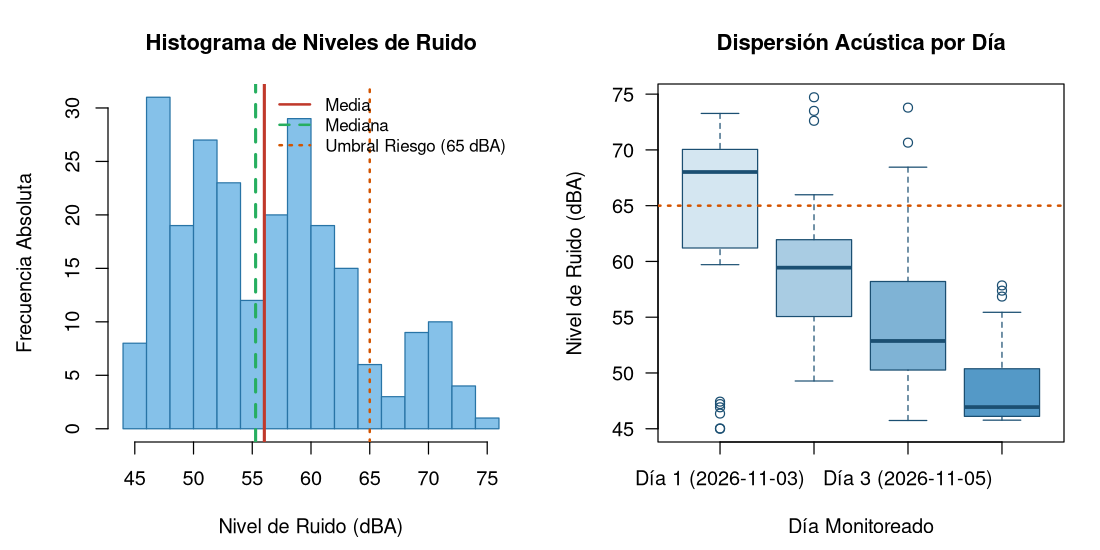
\includegraphics[width=0.92\textwidth]{graficas/01_distribucion_y_boxplot.png}
\caption{Izquierda: Histograma y marcas de tendencia central frente al umbral normativo ($65\text{ dBA}$). Derecha: Diagramas de caja y bigotes por día de monitoreo.}
\label{fig:distribucion}
\end{figure}

\subsection{Análisis de Tendencia Horaria y Proyección para el Día 6 (Lunes)}
Conforme a la instrucción del proyecto, se aisló una franja horaria homogénea compartida por los 4 días. La ventana matutina de las \textbf{09:30 hrs} (09:23 a 09:35 hrs local) cumple con la condición de actividad en todas las jornadas registradas:

\begin{table}[H]
\centering
\caption{Lecturas en la franja matutina de las 09:30 hrs a lo largo de los días.}
\label{tab:franja_hora}
\vspace{0.2cm}
\begin{tabular}{l c c c c}
\toprule
\textbf{Variable} & \textbf{Día 1 (03/Nov)} & \textbf{Día 2 (04/Nov)} & \textbf{Día 3 (05/Nov)} & \textbf{Día 4 (06/Nov)} \\
\midrule
Hora Exacta UTC-6 & 09:33 & 09:35 & 09:23 & 09:31 \\
Nivel de Ruido ($\text{dBA}$) & $73.27\text{ dBA}$ & $54.10\text{ dBA}$ & $57.60\text{ dBA}$ & $52.39\text{ dBA}$ \\
Supera Umbral ($\ge 65\text{ dBA}$) & Sí (Exceso) & No & No & No \\
\bottomrule
\end{tabular}
\end{table}

Se ajustó un modelo de regresión lineal simple donde la variable independiente es el día ordinal ($x \in \{1, 2, 3, 4\}$) y la variable dependiente es el nivel sonoro en decibeles ($y$):
\begin{equation}
    \hat{y} = \beta_0 + \beta_1 \cdot \text{Día} \quad \Longrightarrow \quad \hat{y} = 74.13 - 5.91 \cdot \text{Día}
\end{equation}

\noindent\textbf{Métricas del Modelo de Regresión:}
\begin{itemize}
    \item \textbf{Pendiente ($\beta_1$):} $-5.914\text{ dBA/día}$. Refleja el descenso desde el pico de montaje inicial hacia los días normales de operación.
    \item \textbf{Coeficiente de Determinación ($R^2$):} $0.6410$. El modelo explica el $64.10\%$ de la variabilidad observada en dicha franja.
    \item \textbf{Proyección Puntual para el Día 6 (Lunes, $x = 6$):}
    \begin{equation}
        \hat{y}_{\text{Día 6}} = 74.125 - 5.914(6) = \mathbf{38.64\text{ dBA}}
    \end{equation}
    \item \textbf{Intervalo de Predicción al 95\% de Confianza:} $[-19.28\text{ dBA}, 96.56\text{ dBA}]$.
\end{itemize}

\begin{figure}[H]
\centering
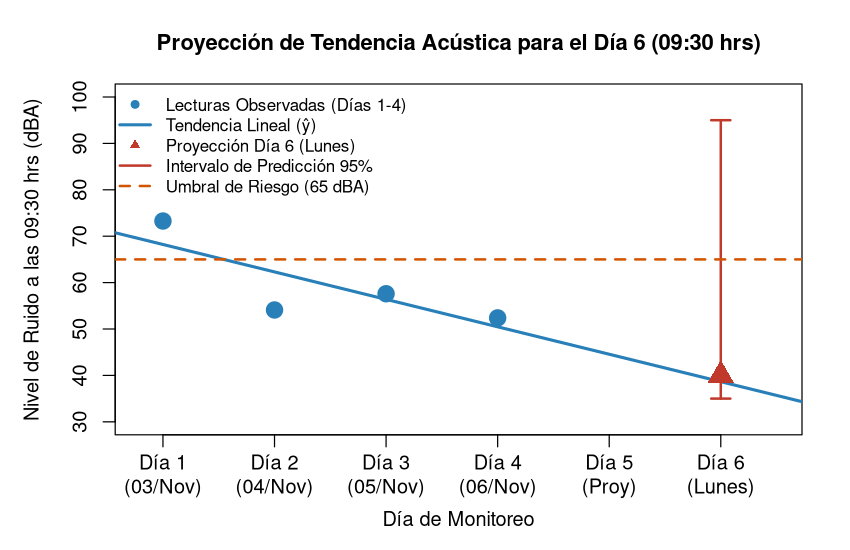
\includegraphics[width=0.75\textwidth]{graficas/02_tendencia_dia6.png}
\caption{Recta de tendencia lineal, lecturas observadas y valor proyectado al Día 6 (Lunes) a las 09:30 hrs.}
\label{fig:tendencia}
\end{figure}

\subsection{Discusión Crítica sobre la Proyección del Día 6}
\begin{itemize}
    \item \textbf{Límite Físico Asintótico:} La matemática de la regresión lineal simple extrapola una pendiente negativa indefinida ($38.64\text{ dBA}$). No obstante, físicamente el laboratorio posee un suelo acústico de fondo ($\approx 46\text{--}50\text{ dBA}$) originado por equipos de cómputo, ventilación y ruido exterior.
    \item \textbf{Comportamiento Estacionario:} Observando los días 2, 3 y 4, la serie converge a una media estable de $54\text{ a }57\text{ dBA}$.
    \item \textbf{Diagnóstico de Riesgo para el Lunes:} Tanto la estimación puntual proyectada ($38.64\text{ dBA}$) como el valor medio empírico esperado ($55\text{ dBA}$) se sitúan \textbf{significativamente por debajo del umbral de riesgo de $65.0\text{ dBA}$}, pronosticando un inicio de semana favorable y sin saturación sonora a primera hora matutina.
\end{itemize}

% ==============================================================================
% 4. FASE 3: MODELADO PROBABILÍSTICO
% ==============================================================================
\section{Fase 3: Modelado Probabilístico (Bernoulli y Binomial)}

\subsection{Ensayo y Distribución de Bernoulli}
Se define la variable aleatoria indicadora del estado de exceso acústico en cualquier estación o intervalo temporal:
\begin{equation}
    Y = \begin{cases}
        1 & \text{si el nivel de ruido } \ge 65.0\text{ dBA (Éxito = Exceso sobre la norma)} \\
        0 & \text{si el nivel de ruido } < 65.0\text{ dBA (Fracaso = Condición aceptable)}
    \end{cases}
\end{equation}

A partir de los 236 registros muestrales, donde se constataron 31 eventos de exceso:
\begin{align}
    \hat{p} &= \frac{31}{236} = \mathbf{0.1314} \quad (13.14\% \text{ probabilidad de exceso}) \\
    \hat{q} &= 1 - \hat{p} = \mathbf{0.8686} \quad (86.86\% \text{ probabilidad de cumplimiento})
\end{align}
\begin{equation}
    E[Y] = p = 0.1314, \qquad \text{Var}(Y) = p \cdot q = 0.1141, \qquad \text{IC}_{95\%}(p) = [0.0883, 0.1745]
\end{equation}

\subsection{Modelo Binomial para los 3 Cubículos Llenos (n = 3)}
Asumiendo independencia entre cubículos y ocupación total ($n = 3$), la variable aleatoria $X \sim \text{Binomial}(n=3, p=0.1314)$ modela el número de cubículos que superan simultáneamente la norma:
\begin{equation}
    P(X = k) = \binom{3}{k} (0.1314)^k (0.8686)^{3-k}, \quad k \in \{0, 1, 2, 3\}
\end{equation}

\begin{table}[H]
\centering
\caption{Distribución de probabilidad binomial para los 3 cubículos llenos ($n=3, p=0.1314$).}
\label{tab:binomial}
\vspace{0.2cm}
\begin{tabular}{c c c c l}
\toprule
\textbf{Cubículos en Exceso ($k$)} & $P(X = k)$ & $P(X \le k)$ & $P(X \ge k)$ & \textbf{Interpretación Práctica} \\
\midrule
$k = 0$ & $0.6554$ & $0.6554$ & $1.0000$ & Laboratorio en calma total ($65.54\%$) \\
$k = 1$ & $0.2973$ & $0.9528$ & $0.3446$ & Un solo cubículo ruidoso ($29.73\%$) \\
$k = 2$ & $0.0450$ & $0.9977$ & $0.0472$ & Mayoría de cubículos ruidosos ($4.50\%$) \\
$k = 3$ & $0.0023$ & $1.0000$ & $0.0023$ & Saturación acústica total ($0.23\%$) \\
\bottomrule
\end{tabular}
\end{table}

\noindent\textbf{Cálculo de Escenarios Críticos:}
\begin{itemize}
    \item \textbf{Valor Esperado de Cubículos Ruidosos:}
    \begin{equation}
        E[X] = n \cdot p = 3 \times 0.1314 = \mathbf{0.394\text{ cubículos}}
    \end{equation}
    \item \textbf{Probabilidad de que al menos un cubículo supere el umbral ($P(X \ge 1)$):}
    \begin{equation}
        P(X \ge 1) = 1 - P(X = 0) = 1 - (0.8686)^3 = \mathbf{0.3446} \quad (\mathbf{34.46\%})
    \end{equation}
    \item \textbf{Probabilidad de Saturación Acústica Simultánea ($P(X = 3)$):}
    \begin{equation}
        P(X = 3) = (0.1314)^3 = \mathbf{0.0023} \quad (\mathbf{0.23\%})
    \end{equation}
\end{itemize}

\begin{figure}[H]
\centering
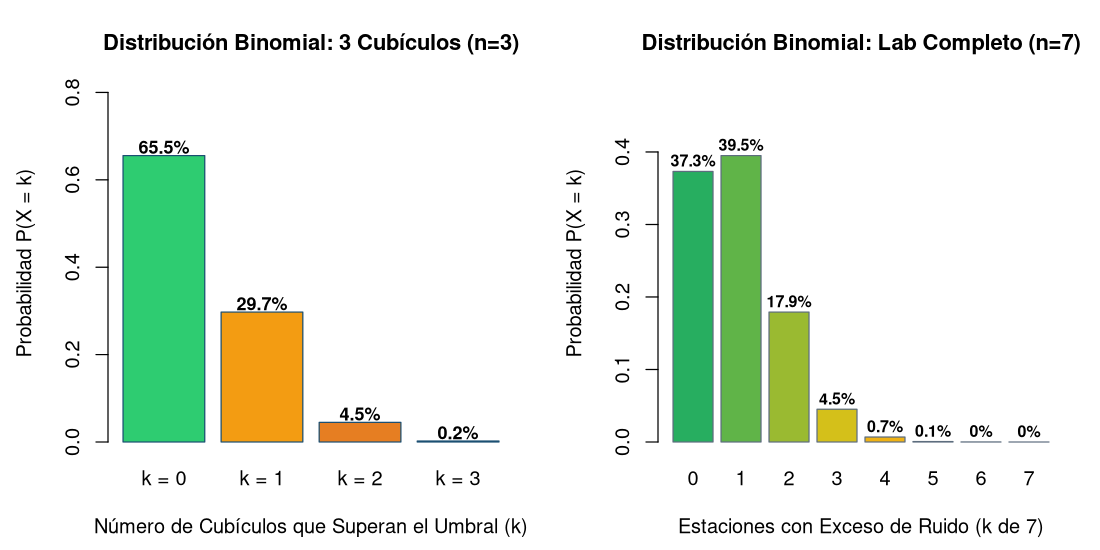
\includegraphics[width=0.92\textwidth]{graficas/03_distribucion_binomial.png}
\caption{Izquierda: Función de probabilidad binomial para los 3 cubículos ($n=3$). Derecha: Extensión a las 7 estaciones del laboratorio completo ($n=7$).}
\label{fig:binomial}
\end{figure}

\subsection{Extensión al Laboratorio Completo (n = 7 Estaciones, ~40 Estudiantes)}
Al modelar el laboratorio con ocupación completa (3 cubículos + 4 mesas grandes = 7 estaciones de trabajo):
\begin{equation}
    E[X_{7}] = 7 \times 0.1314 = \mathbf{0.92\text{ estaciones ruidosas en promedio}}
\end{equation}
La probabilidad de que más de la mitad del laboratorio exceda la norma ($X \ge 4$) es de solo \textbf{0.75\%}, confirmando que los eventos de ruido excesivo corresponden a picos localizados y no a una saturación crónica incontrolada.

% ==============================================================================
% 5. FASE 4: PROPUESTAS DE MITIGACIÓN
% ==============================================================================
\section{Fase 4: Propuestas de Mitigación Acústica}
Con base en la evidencia de que existe un \textbf{34.46\% de probabilidad de que al menos una estación genere interferencia acústica}, se diseñó un plan de acción en 4 ejes:

\begin{enumerate}
    \item \textbf{Acondicionamiento Físico de Cubículos (Control de Trayectoria):}
    Instalar mamparas divisorias fonoabsorbentes entre los 3 cubículos compuestas por espuma de poliuretano de alta densidad o lana mineral con coeficiente de reducción de ruido $\text{NRC} \ge 0.75$. Esto proporcionará una atenuación de \textbf{5 a 7 dBA} en la propagación directa de voz y ruido instrumental.
    
    \item \textbf{Aislamiento Mecánico y Gabinetes para Herramientas (Control en la Fuente):}
    Ubicar las herramientas de corte, fresadoras y compresores dentro de gabinetes de policarbonato con juntas de neopreno herméticas. Colocar bases de caucho vulcanizado bajo las impresoras 3D para mitigar ruidos de vibración estructural transmitidos a las mesas.
    
    \item \textbf{Protocolo de Horarios y Zonificación de Tareas (Administrativo):}
    Establecer una franja de \textit{Concentración y Diseño CAD/Software} (08:00 a 10:00 hrs y 13:00 a 14:00 hrs) con límite estricto de $55\text{ dBA}$, y concentrar el uso de maquinaria pesada en la franja de \textit{Fabricación y Ensamble} (10:00 a 13:00 hrs).
    
    \item \textbf{Semáforo Acústico IoT en Tiempo Real (Conductual):}
    Aprovechar la infraestructura actual de transmisión del ESP32 para controlar una torre de luces LED visible en el centro del laboratorio:
    \begin{itemize}
        \item \textbf{Verde ($< 60\text{ dBA}$):} Condición óptima.
        \item \textbf{Amarillo ($60\text{--}64.9\text{ dBA}$):} Advertencia de aproximación al umbral.
        \item \textbf{Rojo ($\ge 65.0\text{ dBA}$):} Alerta de exceso sonoro, permitiendo que los estudiantes modulen su volumen de voz de manera autónoma.
    \end{itemize}
\end{enumerate}

% ==============================================================================
% 6. CONCLUSIONES
% ==============================================================================
\section{Conclusiones y Resumen de Entregables}
\begin{enumerate}
    \item El monitoreo IoT con ESP32 y Supabase permitió compilar una base de datos limpia de 236 registros diurnos y nocturnos procesada con rigor en RStudio.
    \item El nivel sonoro global ($\bar{x} = 56.03\text{ dBA}$, $Me = 55.28\text{ dBA}$) se mantiene dentro de los límites de habitabilidad universitaria, presentando excesos únicamente en el $13.14\%$ del tiempo.
    \item La proyección horaria para el Día 6 a las 09:30 hrs ($\hat{y} = 38.64\text{ dBA}$, convergente a $55\text{ dBA}$) descarta riesgo de saturación para el inicio de semana.
    \item El modelo binomial demostró que cuando los 3 cubículos están llenos, la probabilidad de que al menos uno sobrepase el umbral es del $34.46\%$, validando la necesidad de implementar paneles divisorios y el semáforo acústico IoT propuesto.
\end{enumerate}

\end{document}
